% Options for packages loaded elsewhere
\PassOptionsToPackage{unicode}{hyperref}
\PassOptionsToPackage{hyphens}{url}
%
\documentclass[
]{article}
\usepackage{amsmath,amssymb}
\usepackage{lmodern}
\usepackage{iftex}
\ifPDFTeX
  \usepackage[T1]{fontenc}
  \usepackage[utf8]{inputenc}
  \usepackage{textcomp} % provide euro and other symbols
\else % if luatex or xetex
  \usepackage{unicode-math}
  \defaultfontfeatures{Scale=MatchLowercase}
  \defaultfontfeatures[\rmfamily]{Ligatures=TeX,Scale=1}
\fi
% Use upquote if available, for straight quotes in verbatim environments
\IfFileExists{upquote.sty}{\usepackage{upquote}}{}
\IfFileExists{microtype.sty}{% use microtype if available
  \usepackage[]{microtype}
  \UseMicrotypeSet[protrusion]{basicmath} % disable protrusion for tt fonts
}{}
\makeatletter
\@ifundefined{KOMAClassName}{% if non-KOMA class
  \IfFileExists{parskip.sty}{%
    \usepackage{parskip}
  }{% else
    \setlength{\parindent}{0pt}
    \setlength{\parskip}{6pt plus 2pt minus 1pt}}
}{% if KOMA class
  \KOMAoptions{parskip=half}}
\makeatother
\usepackage{xcolor}
\usepackage[margin=1in]{geometry}
\usepackage{color}
\usepackage{fancyvrb}
\newcommand{\VerbBar}{|}
\newcommand{\VERB}{\Verb[commandchars=\\\{\}]}
\DefineVerbatimEnvironment{Highlighting}{Verbatim}{commandchars=\\\{\}}
% Add ',fontsize=\small' for more characters per line
\usepackage{framed}
\definecolor{shadecolor}{RGB}{248,248,248}
\newenvironment{Shaded}{\begin{snugshade}}{\end{snugshade}}
\newcommand{\AlertTok}[1]{\textcolor[rgb]{0.94,0.16,0.16}{#1}}
\newcommand{\AnnotationTok}[1]{\textcolor[rgb]{0.56,0.35,0.01}{\textbf{\textit{#1}}}}
\newcommand{\AttributeTok}[1]{\textcolor[rgb]{0.77,0.63,0.00}{#1}}
\newcommand{\BaseNTok}[1]{\textcolor[rgb]{0.00,0.00,0.81}{#1}}
\newcommand{\BuiltInTok}[1]{#1}
\newcommand{\CharTok}[1]{\textcolor[rgb]{0.31,0.60,0.02}{#1}}
\newcommand{\CommentTok}[1]{\textcolor[rgb]{0.56,0.35,0.01}{\textit{#1}}}
\newcommand{\CommentVarTok}[1]{\textcolor[rgb]{0.56,0.35,0.01}{\textbf{\textit{#1}}}}
\newcommand{\ConstantTok}[1]{\textcolor[rgb]{0.00,0.00,0.00}{#1}}
\newcommand{\ControlFlowTok}[1]{\textcolor[rgb]{0.13,0.29,0.53}{\textbf{#1}}}
\newcommand{\DataTypeTok}[1]{\textcolor[rgb]{0.13,0.29,0.53}{#1}}
\newcommand{\DecValTok}[1]{\textcolor[rgb]{0.00,0.00,0.81}{#1}}
\newcommand{\DocumentationTok}[1]{\textcolor[rgb]{0.56,0.35,0.01}{\textbf{\textit{#1}}}}
\newcommand{\ErrorTok}[1]{\textcolor[rgb]{0.64,0.00,0.00}{\textbf{#1}}}
\newcommand{\ExtensionTok}[1]{#1}
\newcommand{\FloatTok}[1]{\textcolor[rgb]{0.00,0.00,0.81}{#1}}
\newcommand{\FunctionTok}[1]{\textcolor[rgb]{0.00,0.00,0.00}{#1}}
\newcommand{\ImportTok}[1]{#1}
\newcommand{\InformationTok}[1]{\textcolor[rgb]{0.56,0.35,0.01}{\textbf{\textit{#1}}}}
\newcommand{\KeywordTok}[1]{\textcolor[rgb]{0.13,0.29,0.53}{\textbf{#1}}}
\newcommand{\NormalTok}[1]{#1}
\newcommand{\OperatorTok}[1]{\textcolor[rgb]{0.81,0.36,0.00}{\textbf{#1}}}
\newcommand{\OtherTok}[1]{\textcolor[rgb]{0.56,0.35,0.01}{#1}}
\newcommand{\PreprocessorTok}[1]{\textcolor[rgb]{0.56,0.35,0.01}{\textit{#1}}}
\newcommand{\RegionMarkerTok}[1]{#1}
\newcommand{\SpecialCharTok}[1]{\textcolor[rgb]{0.00,0.00,0.00}{#1}}
\newcommand{\SpecialStringTok}[1]{\textcolor[rgb]{0.31,0.60,0.02}{#1}}
\newcommand{\StringTok}[1]{\textcolor[rgb]{0.31,0.60,0.02}{#1}}
\newcommand{\VariableTok}[1]{\textcolor[rgb]{0.00,0.00,0.00}{#1}}
\newcommand{\VerbatimStringTok}[1]{\textcolor[rgb]{0.31,0.60,0.02}{#1}}
\newcommand{\WarningTok}[1]{\textcolor[rgb]{0.56,0.35,0.01}{\textbf{\textit{#1}}}}
\usepackage{graphicx}
\makeatletter
\def\maxwidth{\ifdim\Gin@nat@width>\linewidth\linewidth\else\Gin@nat@width\fi}
\def\maxheight{\ifdim\Gin@nat@height>\textheight\textheight\else\Gin@nat@height\fi}
\makeatother
% Scale images if necessary, so that they will not overflow the page
% margins by default, and it is still possible to overwrite the defaults
% using explicit options in \includegraphics[width, height, ...]{}
\setkeys{Gin}{width=\maxwidth,height=\maxheight,keepaspectratio}
% Set default figure placement to htbp
\makeatletter
\def\fps@figure{htbp}
\makeatother
\setlength{\emergencystretch}{3em} % prevent overfull lines
\providecommand{\tightlist}{%
  \setlength{\itemsep}{0pt}\setlength{\parskip}{0pt}}
\setcounter{secnumdepth}{-\maxdimen} % remove section numbering
\ifLuaTeX
  \usepackage{selnolig}  % disable illegal ligatures
\fi
\IfFileExists{bookmark.sty}{\usepackage{bookmark}}{\usepackage{hyperref}}
\IfFileExists{xurl.sty}{\usepackage{xurl}}{} % add URL line breaks if available
\urlstyle{same} % disable monospaced font for URLs
\hypersetup{
  pdftitle={HUDM6026 Homework\_07 In-class Activity},
  pdfauthor={Chenguang Pan \& Seng Lei},
  hidelinks,
  pdfcreator={LaTeX via pandoc}}

\title{HUDM6026 Homework\_07 In-class Activity}
\author{Chenguang Pan \& Seng Lei}
\date{Mar 22, 2023}

\begin{document}
\maketitle

\hypertarget{part-1}{%
\subsection{Part 1}\label{part-1}}

\emph{Your group work will involve the acupuncture data set. I've
uploaded a csv file in the Misc folder in the Files section.}

\emph{Data for this group work come from a randomized experiment to
study the efficacy of acupuncture for treating headaches. Results of the
trial were published in the British Medical Journal in 2004. You may
view the paper at the following
link:\url{http://www.bmj.com/content/328/7442/744.full} The data set
includes 301 cases, 140 control (no acupuncture) and 161 treated
(acupuncture). Participants were randomly assigned to groups. Variable
names and descriptions are as follows:age; age in years sex; male = 0,
female = 1 migraine; diagnosis of migraines = 1, diagnosis of
tension-type headaches = 0 chronicity; number of years of headache
disorder at baseline acupuncturist; ID for acupuncture provider group;
acupuncture treatment group = 1, control group = 0 pk1; headache
severity rating at baseline pk5; headache severity rating 1 year later}

\emph{Your task in group work today is to be done in three parts.}

\emph{Part 1 is to run the standard two-sample t-test to test if
acupuncture significantly decreased headache pain in study participants.
Explore the assumptions of the t-test by examining the data through
graphs.}

\textbf{MY SOLUTION}

\begin{Shaded}
\begin{Highlighting}[]
\SpecialCharTok{\textgreater{}} \CommentTok{\# load the dataset}
\ErrorTok{\textgreater{}}\NormalTok{ df }\OtherTok{\textless{}{-}} \FunctionTok{read.csv}\NormalTok{(}\StringTok{"acupuncture.csv"}\NormalTok{)}
\SpecialCharTok{\textgreater{}} \FunctionTok{head}\NormalTok{(df)}
\NormalTok{   id age sex migraine chronicity acupuncturist group   pk1      pk5 remission}
\DecValTok{1} \DecValTok{104}  \DecValTok{32}   \DecValTok{1}        \DecValTok{1}         \DecValTok{14}            \DecValTok{12}     \DecValTok{0} \FloatTok{16.00} \FloatTok{15.33333}         \DecValTok{0}
\DecValTok{2} \DecValTok{108}  \DecValTok{56}   \DecValTok{1}        \DecValTok{1}         \DecValTok{40}             \DecValTok{9}     \DecValTok{0} \FloatTok{16.50} \FloatTok{23.25000}         \DecValTok{0}
\DecValTok{3} \DecValTok{112}  \DecValTok{45}   \DecValTok{1}        \DecValTok{1}         \DecValTok{27}             \DecValTok{9}     \DecValTok{1}  \FloatTok{9.25}  \FloatTok{6.25000}         \DecValTok{1}
\DecValTok{4} \DecValTok{113}  \DecValTok{45}   \DecValTok{1}        \DecValTok{1}         \DecValTok{30}             \DecValTok{9}     \DecValTok{1} \FloatTok{42.50} \FloatTok{51.25000}         \DecValTok{0}
\DecValTok{5} \DecValTok{114}  \DecValTok{49}   \DecValTok{1}        \DecValTok{1}         \DecValTok{49}             \DecValTok{9}     \DecValTok{1} \FloatTok{24.25} \FloatTok{25.25000}         \DecValTok{0}
\DecValTok{6} \DecValTok{126}  \DecValTok{47}   \DecValTok{1}        \DecValTok{1}         \DecValTok{42}             \DecValTok{5}     \DecValTok{0} \FloatTok{21.00} \FloatTok{15.25000}         \DecValTok{0}
\SpecialCharTok{\textgreater{}} 
\ErrorTok{\textgreater{}} \CommentTok{\# subset the treatment and control group}
\ErrorTok{\textgreater{}}\NormalTok{ group\_treat }\OtherTok{\textless{}{-}}\NormalTok{ df}\SpecialCharTok{$}\NormalTok{pk5[}\FunctionTok{which}\NormalTok{(df}\SpecialCharTok{$}\NormalTok{group}\SpecialCharTok{==}\DecValTok{1}\NormalTok{)]}
\SpecialCharTok{\textgreater{}}\NormalTok{ group\_control }\OtherTok{\textless{}{-}}\NormalTok{ df}\SpecialCharTok{$}\NormalTok{pk5[}\FunctionTok{which}\NormalTok{(df}\SpecialCharTok{$}\NormalTok{group}\SpecialCharTok{==}\DecValTok{0}\NormalTok{)]}
\SpecialCharTok{\textgreater{}} 
\ErrorTok{\textgreater{}} \CommentTok{\# draw the graph of treatment and control group\textquotesingle{}s effect}
\ErrorTok{\textgreater{}} \FunctionTok{library}\NormalTok{(tidyverse)}
\SpecialCharTok{\textgreater{}} \FunctionTok{par}\NormalTok{(}\AttributeTok{mfrow=}\FunctionTok{c}\NormalTok{(}\DecValTok{1}\NormalTok{, }\DecValTok{2}\NormalTok{))}
\SpecialCharTok{\textgreater{}}\NormalTok{ df }\SpecialCharTok{\%\textgreater{}\%} \FunctionTok{ggplot}\NormalTok{(}\FunctionTok{aes}\NormalTok{(}\AttributeTok{x =} \FunctionTok{factor}\NormalTok{(group), }\AttributeTok{y =}\NormalTok{ pk5)) }\SpecialCharTok{+} 
\SpecialCharTok{+}   \FunctionTok{geom\_boxplot}\NormalTok{()}
\SpecialCharTok{\textgreater{}}\NormalTok{ df }\SpecialCharTok{\%\textgreater{}\%} \FunctionTok{ggplot}\NormalTok{(}\FunctionTok{aes}\NormalTok{(}\AttributeTok{x =}\NormalTok{ pk5),) }\SpecialCharTok{+}
\SpecialCharTok{+}   \FunctionTok{geom\_density}\NormalTok{(}\FunctionTok{aes}\NormalTok{(}\AttributeTok{color =} \FunctionTok{factor}\NormalTok{(group)))}
\end{Highlighting}
\end{Shaded}

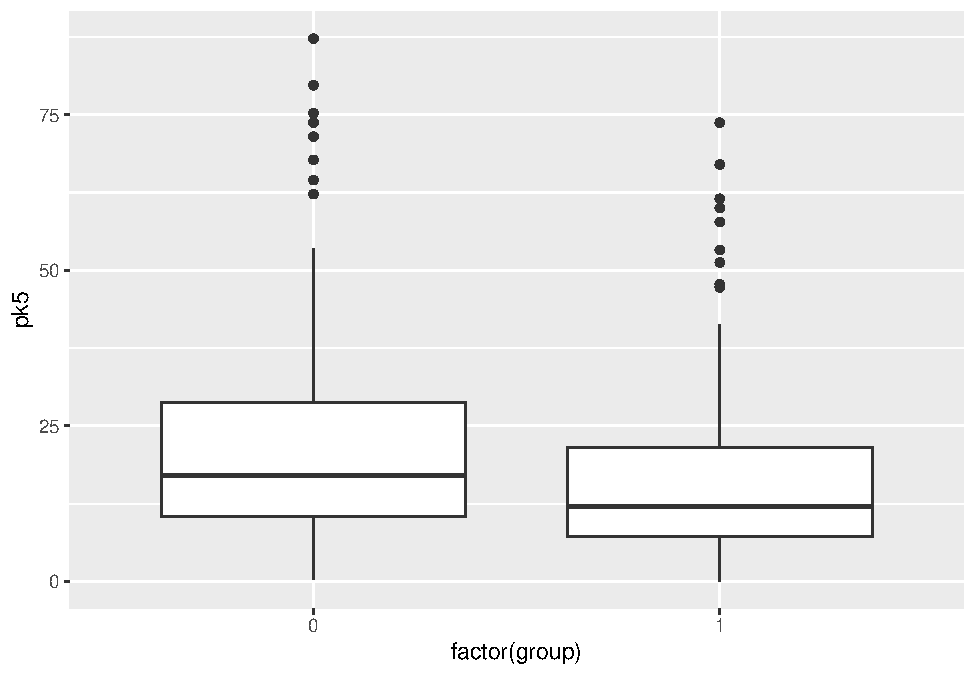
\includegraphics[width=0.5\linewidth,height=0.25\textheight]{Homework_07_new_Pan_files/figure-latex/unnamed-chunk-1-1}
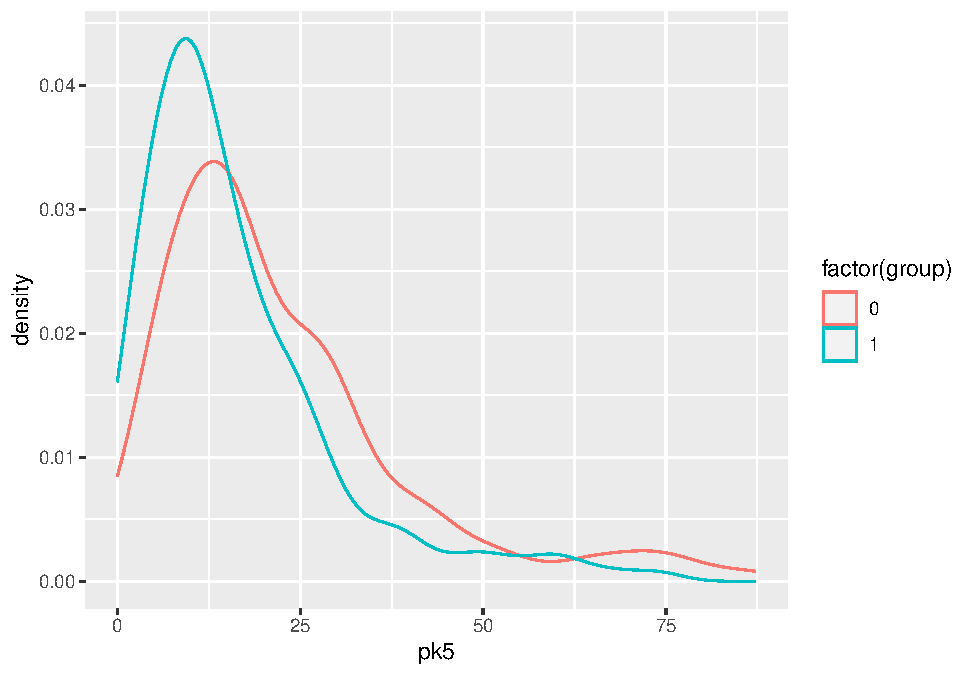
\includegraphics[width=0.5\linewidth,height=0.25\textheight]{Homework_07_new_Pan_files/figure-latex/unnamed-chunk-1-2}
From the graphs we can see that the treatment group has lower average
PK5 than control group. Next, I run the two-sample t-test and turn the
argument \texttt{var.equal} to \texttt{FALSE}, although Levene's Test
shows that there is no significant difference between the two groups'
variance.

\begin{Shaded}
\begin{Highlighting}[]
\SpecialCharTok{\textgreater{}} \CommentTok{\# run the two{-}sample t{-}test}
\ErrorTok{\textgreater{}} \FunctionTok{t.test}\NormalTok{(group\_treat, group\_control,}\AttributeTok{var.equal =} \ConstantTok{FALSE}\NormalTok{)}

\NormalTok{    Welch Two Sample t}\SpecialCharTok{{-}}\NormalTok{test}

\NormalTok{data}\SpecialCharTok{:}\NormalTok{  group\_treat and group\_control}
\NormalTok{t }\OtherTok{=} \SpecialCharTok{{-}}\FloatTok{3.3892}\NormalTok{, df }\OtherTok{=} \FloatTok{266.6}\NormalTok{, p}\SpecialCharTok{{-}}\NormalTok{value }\OtherTok{=} \FloatTok{0.0008069}
\NormalTok{alternative hypothesis}\SpecialCharTok{:}\NormalTok{ true difference }\ControlFlowTok{in}\NormalTok{ means is not equal to }\DecValTok{0}
\DecValTok{95}\NormalTok{ percent confidence interval}\SpecialCharTok{:}
 \SpecialCharTok{{-}}\FloatTok{9.638399} \SpecialCharTok{{-}}\FloatTok{2.554924}
\NormalTok{sample estimates}\SpecialCharTok{:}
\NormalTok{mean of x mean of y }
 \FloatTok{16.24679}  \FloatTok{22.34345} 
\end{Highlighting}
\end{Shaded}

The Welch two sample t-test shows that there is statistically
significant difference in two groups' average effect on \texttt{PK5},
\(t(266.6)=-3.389\) and \(p <.001\).\\
In addition, I checked the baseline balance on \texttt{PK1} to ensure
that we can use \texttt{PK5} to ensure the ramdomization worked as
intended.

\begin{Shaded}
\begin{Highlighting}[]
\SpecialCharTok{\textgreater{}} \CommentTok{\# install the package to run Cohen\textquotesingle{}s d}
\ErrorTok{\textgreater{}} \CommentTok{\# install.packages("lsr")}
\ErrorTok{\textgreater{}} \FunctionTok{library}\NormalTok{(lsr)}
\SpecialCharTok{\textgreater{}} \CommentTok{\# extract the treatment and control group at baseline}
\ErrorTok{\textgreater{}}\NormalTok{ basegroup\_treat }\OtherTok{\textless{}{-}}\NormalTok{ df}\SpecialCharTok{$}\NormalTok{pk1[}\FunctionTok{which}\NormalTok{(df}\SpecialCharTok{$}\NormalTok{group}\SpecialCharTok{==}\DecValTok{1}\NormalTok{)]}
\SpecialCharTok{\textgreater{}}\NormalTok{ basegroup\_control }\OtherTok{\textless{}{-}}\NormalTok{ df}\SpecialCharTok{$}\NormalTok{pk1[}\FunctionTok{which}\NormalTok{(df}\SpecialCharTok{$}\NormalTok{group}\SpecialCharTok{==}\DecValTok{0}\NormalTok{)]}
\SpecialCharTok{\textgreater{}} \CommentTok{\# calculate the cohen\textquotesingle{}s d to check the balance}
\ErrorTok{\textgreater{}} \FunctionTok{cohensD}\NormalTok{(basegroup\_treat,basegroup\_control)}
\NormalTok{[}\DecValTok{1}\NormalTok{] }\FloatTok{0.1384973}
\end{Highlighting}
\end{Shaded}

The results show that the value of Cohen's D at baseline is .14, larger
than .1 but fewer than .2. As a rule of thumb introduced by Maxwell et
al.(2018), this result might cause some concern but not problematic.
Further scrutiny is necessary. I also compare the ratio of group
variance at baseline.

\begin{Shaded}
\begin{Highlighting}[]
\SpecialCharTok{\textgreater{}} \CommentTok{\# check the ratio of group variance for two groups at baseline}
\ErrorTok{\textgreater{}}\NormalTok{ ratio\_of\_variance }\OtherTok{\textless{}{-}} \FunctionTok{var}\NormalTok{(basegroup\_treat)}\SpecialCharTok{/}\FunctionTok{var}\NormalTok{(basegroup\_control)}
\SpecialCharTok{\textgreater{}}\NormalTok{ ratio\_of\_variance}
\NormalTok{[}\DecValTok{1}\NormalTok{] }\FloatTok{0.7079415}
\end{Highlighting}
\end{Shaded}

The ratio is smaller than .8, which may also be a sign of concern. As
Prof.~Keller's instruction in HUDM5123, we need to continue to check the
covariates balance at baseline. But I ignored this issue and moved to
the next task here.

\hypertarget{part-2}{%
\subsection{Part 2}\label{part-2}}

\emph{Part 2 is to identify a non-standard test statistic that your team
suspects will also be sensitive to departures from the null hypothesis
of no treatment effect. leveene's test of the variance ratio or
correlation pk1-pk5 in treatment/ pk1-pk5 in control rank all the data
in pk5}

\textbf{MY SOLUTION}\\
First, I test the normality of two groups' distributions on
\texttt{PK5}.

\begin{Shaded}
\begin{Highlighting}[]
\SpecialCharTok{\textgreater{}} \CommentTok{\# to test the normality of the two distribution}
\ErrorTok{\textgreater{}} \FunctionTok{shapiro.test}\NormalTok{(group\_treat)}

\NormalTok{    Shapiro}\SpecialCharTok{{-}}\NormalTok{Wilk normality test}

\NormalTok{data}\SpecialCharTok{:}\NormalTok{  group\_treat}
\NormalTok{W }\OtherTok{=} \FloatTok{0.83345}\NormalTok{, p}\SpecialCharTok{{-}}\NormalTok{value }\OtherTok{=} \FloatTok{2.928e{-}12}
\SpecialCharTok{\textgreater{}} \FunctionTok{shapiro.test}\NormalTok{(group\_control)}

\NormalTok{    Shapiro}\SpecialCharTok{{-}}\NormalTok{Wilk normality test}

\NormalTok{data}\SpecialCharTok{:}\NormalTok{  group\_control}
\NormalTok{W }\OtherTok{=} \FloatTok{0.84781}\NormalTok{, p}\SpecialCharTok{{-}}\NormalTok{value }\OtherTok{=} \FloatTok{1.017e{-}10}
\SpecialCharTok{\textgreater{}} \CommentTok{\# draw the qq plot}
\ErrorTok{\textgreater{}}\NormalTok{ mfrow}\OtherTok{=}\FunctionTok{c}\NormalTok{(}\DecValTok{1}\NormalTok{,}\DecValTok{2}\NormalTok{)}
\SpecialCharTok{\textgreater{}} \FunctionTok{qqnorm}\NormalTok{(group\_treat)}
\SpecialCharTok{\textgreater{}} \FunctionTok{qqline}\NormalTok{(group\_treat)}
\SpecialCharTok{\textgreater{}} \FunctionTok{qqnorm}\NormalTok{(group\_control)}
\SpecialCharTok{\textgreater{}} \FunctionTok{qqline}\NormalTok{(group\_control)}
\end{Highlighting}
\end{Shaded}

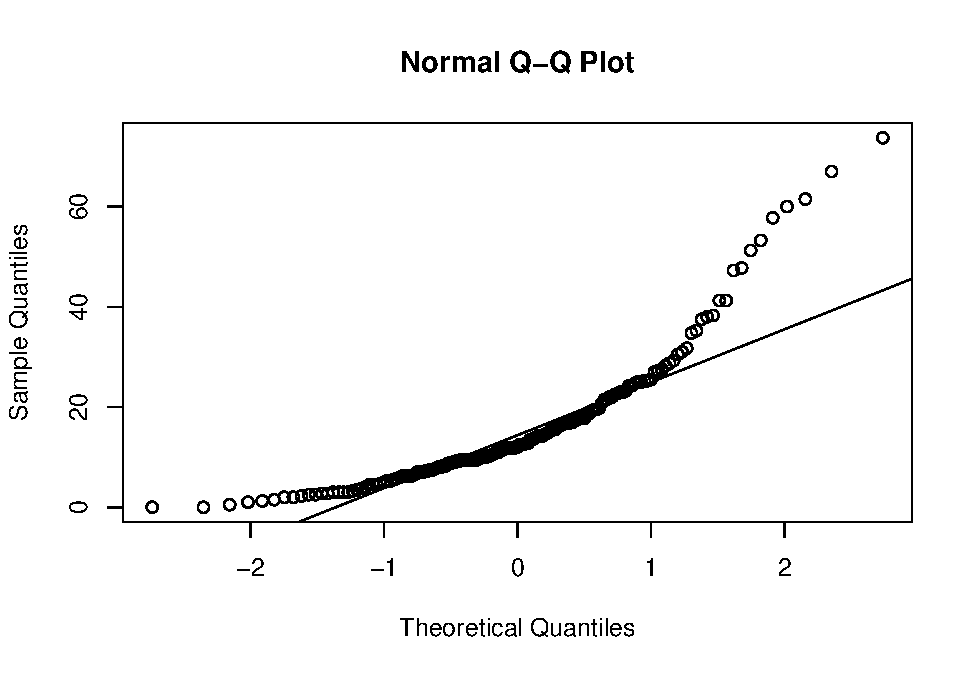
\includegraphics[width=0.5\linewidth,height=0.5\textheight]{Homework_07_new_Pan_files/figure-latex/unnamed-chunk-5-1}
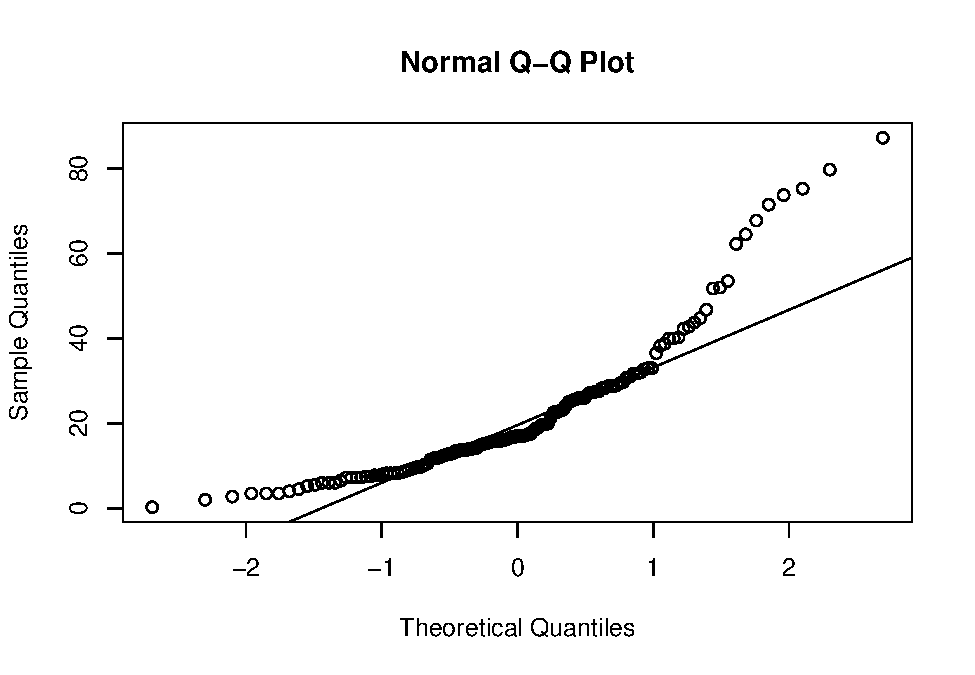
\includegraphics[width=0.5\linewidth,height=0.5\textheight]{Homework_07_new_Pan_files/figure-latex/unnamed-chunk-5-2}
The Shapiro-Wilk Test and the Q-Q plot indicate that the both groups are
not follow the normal distribution. From the original distribution graph
made in the Part 1, one can see both distributions are positively
skewed.

Therefore, running the regular two-sample T test in Part-1 may not a
good choice since it compares the central tendency by using means and
this statistic might be influenced by the extreme values.

We decided to choose the ranked-based test,i.e., the Wilcoxon rank-sum
test, which is more robust to departures from normality since this test
use median rather than mean to represent the central tendency and median
is less sensitive to extreme values.

\begin{Shaded}
\begin{Highlighting}[]
\SpecialCharTok{\textgreater{}}\NormalTok{ obs\_test\_resulst }\OtherTok{\textless{}{-}} \FunctionTok{wilcox.test}\NormalTok{(group\_treat, group\_control, }\AttributeTok{alternative =} \StringTok{"two.sided"}\NormalTok{)}
\SpecialCharTok{\textgreater{}}\NormalTok{ obs\_test\_resulst}

\NormalTok{    Wilcoxon rank sum test with continuity correction}

\NormalTok{data}\SpecialCharTok{:}\NormalTok{  group\_treat and group\_control}
\NormalTok{W }\OtherTok{=} \DecValTok{8392}\NormalTok{, p}\SpecialCharTok{{-}}\NormalTok{value }\OtherTok{=} \FloatTok{0.000133}
\NormalTok{alternative hypothesis}\SpecialCharTok{:}\NormalTok{ true location shift is not equal to }\DecValTok{0}
\end{Highlighting}
\end{Shaded}

The Wilcoxon rank-sum test's result presents that the two groups'
medians are significantly different, \(p < .001\). The two groups have
different distributions.

\hypertarget{part-3}{%
\subsection{Part 3}\label{part-3}}

\emph{Part 3 is to use the non-standard test statistic in a permutation
framework to determine the approximate significance level (p-value).}

\textbf{MY SOLUTION}

\begin{Shaded}
\begin{Highlighting}[]
\SpecialCharTok{\textgreater{}} \FunctionTok{library}\NormalTok{(boot)}
\SpecialCharTok{\textgreater{}} 
\ErrorTok{\textgreater{}} \CommentTok{\# write a function to conduct the Wilcoxon rank{-}sum test}
\ErrorTok{\textgreater{}}\NormalTok{ median\_diff }\OtherTok{\textless{}{-}} \ControlFlowTok{function}\NormalTok{(dat, index) \{}
\SpecialCharTok{+}   \CommentTok{\# fix the group assignments}
\SpecialCharTok{+}\NormalTok{   treat\_or\_not }\OtherTok{\textless{}{-}}\NormalTok{ dat}\SpecialCharTok{$}\NormalTok{group}
\SpecialCharTok{+}   \CommentTok{\# permute the pk5 (combined data)}
\SpecialCharTok{+}\NormalTok{   pk5 }\OtherTok{\textless{}{-}}\NormalTok{ dat}\SpecialCharTok{$}\NormalTok{pk5[index]}
\SpecialCharTok{+}   \CommentTok{\# extract the treat and control groups}
\SpecialCharTok{+}\NormalTok{   treat }\OtherTok{\textless{}{-}}\NormalTok{ pk5[}\FunctionTok{which}\NormalTok{(treat\_or\_not}\SpecialCharTok{==}\DecValTok{1}\NormalTok{)]}
\SpecialCharTok{+}\NormalTok{   control }\OtherTok{\textless{}{-}}\NormalTok{ pk5[}\FunctionTok{which}\NormalTok{(treat\_or\_not}\SpecialCharTok{==}\DecValTok{0}\NormalTok{)]}
\SpecialCharTok{+}   \CommentTok{\# run the Wilcoxon rank{-}sum test to get the statistic}
\SpecialCharTok{+}\NormalTok{   test\_out }\OtherTok{\textless{}{-}} \FunctionTok{median}\NormalTok{(treat}\SpecialCharTok{{-}}\NormalTok{control)}
\SpecialCharTok{+}   \FunctionTok{return}\NormalTok{(test\_out)}
\SpecialCharTok{+}\NormalTok{ \}}
\SpecialCharTok{\textgreater{}} 
\ErrorTok{\textgreater{}} 
\ErrorTok{\textgreater{}}\NormalTok{ boot\_out }\OtherTok{\textless{}{-}} \FunctionTok{boot}\NormalTok{(}\AttributeTok{data =}\NormalTok{ df, }
\SpecialCharTok{+}                  \AttributeTok{statistic =}\NormalTok{ median\_diff, }
\SpecialCharTok{+}                  \AttributeTok{R =} \DecValTok{10000}\NormalTok{, }\AttributeTok{sim =} \StringTok{"permutation"}\NormalTok{)}
\SpecialCharTok{\textgreater{}} \CommentTok{\# use the observed statistic got from the part}
\ErrorTok{\textgreater{}} \FunctionTok{hist}\NormalTok{(boot\_out}\SpecialCharTok{$}\NormalTok{t, }\DecValTok{50}\NormalTok{)}
\end{Highlighting}
\end{Shaded}

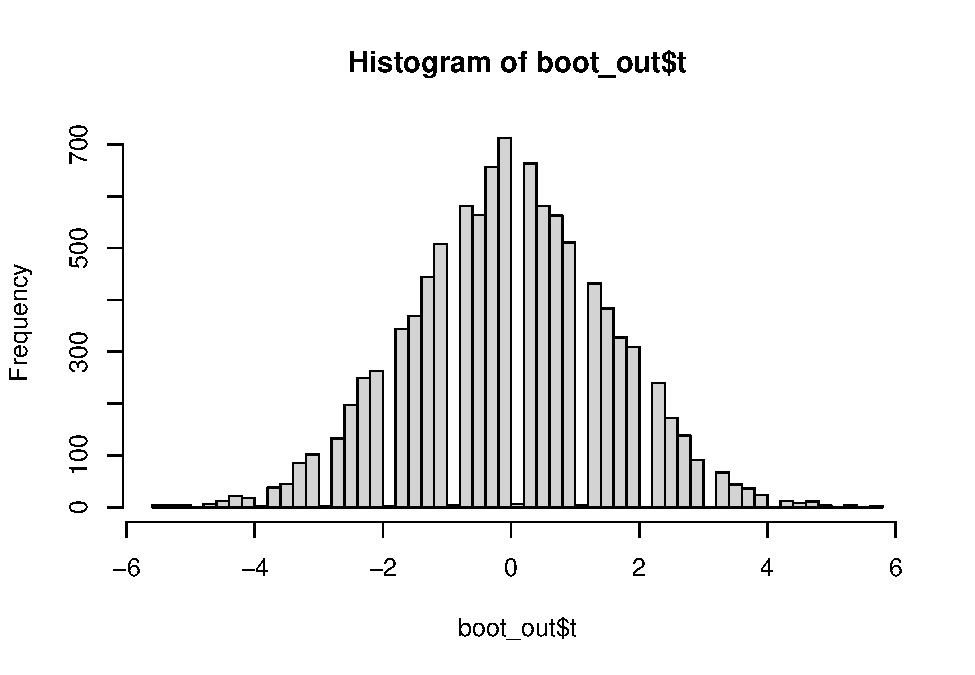
\includegraphics{Homework_07_new_Pan_files/figure-latex/unnamed-chunk-7-1.pdf}

\begin{Shaded}
\begin{Highlighting}[]
\SpecialCharTok{\textgreater{}}\NormalTok{ p\_value }\OtherTok{\textless{}{-}} \FunctionTok{length}\NormalTok{(}\FunctionTok{which}\NormalTok{(}\FunctionTok{abs}\NormalTok{(boot\_out}\SpecialCharTok{$}\NormalTok{t) }\SpecialCharTok{\textgreater{}=} \FunctionTok{abs}\NormalTok{(boot\_out}\SpecialCharTok{$}\NormalTok{t0)))}\SpecialCharTok{/} \FunctionTok{length}\NormalTok{(boot\_out}\SpecialCharTok{$}\NormalTok{t)}
\SpecialCharTok{\textgreater{}}\NormalTok{ p\_value}
\NormalTok{[}\DecValTok{1}\NormalTok{] }\FloatTok{0.0055}
\end{Highlighting}
\end{Shaded}

The permutation result indicates that the difference in medians is still
statistically significant , \emph{p}=0.0055.

\end{document}
